\documentclass[aps,prb,twocolumn,floatfix,nofootinbib,superscriptaddress]{revtex4-2}

\usepackage{amsmath,amssymb,bm}
\usepackage{booktabs}
\usepackage{graphicx}
\usepackage[colorlinks=true,linkcolor=blue,citecolor=blue,urlcolor=blue]{hyperref}
\usepackage{microtype}

\newcommand{\Tr}{\operatorname{Tr}}
\newcommand{\E}{\mathbb{E}}

\begin{document}

\title{Resolved-record many-body Lyapunov analysis at four circumferences:
hard and soft adaptive chiral domain walls}

\author{Asadullah Bhuiyan}
\date{September 9, 2026}

\begin{abstract}
We analyze 600 independent maximally mixed Gaussian Born trajectories of the
adaptive chiral circuit at $N_x=20$, $N_y=20,30,40$, and depth $T=4N_y$.
The hard support-truncated arm and corrected soft untruncated arm each contain
$S=100$ trajectories per circumference.  The saved one-particle occupations
fix the normalized many-body singular spectrum, while the cumulative realized
Born log probability restores its absolute normalization.  All 120 result and
completion pairs pass the server-pinned byte-count, SHA-256, configuration,
source, event-count, and numerical checks.  The leading rate $\lambda_0$ is
stable between $[2N_y,3N_y]$ and $[3N_y,4N_y]$ at every size, and its
same-window agreement with the record-weight slope is better than
$1.8\times10^{-5}$ relatively.  This repairs the temporal failure of the
earlier $2N_y$ pilot.  It does not, however, produce a controlled CFT
coefficient: the three-size $1/N_y^2$ coefficients have bootstrap intervals
containing zero and order-unity sensitivity to fit form.  Moreover, late
soft-wall excited levels are mostly below the double-precision occupation
resolution.  The data establish absolute-spectrum reconstruction, leading-rate
convergence, and wall-localized residual purification, but not a precision
$c_{\rm eff}$ or labeled operator spectrum.
\end{abstract}

\maketitle

\section{Question and completed ensemble}

For a resolved measurement record $\bm m$, the monitored circuit defines a
many-body evolution operator (mEO) $\hat V_{\bm m}(t)$.  We ask whether the
new $T=4N_y$ purification ensemble is deep enough to extract its leading
many-body Lyapunov rates and the finite-size coefficients used by Zabalo
\emph{et al.}\ [arXiv:2107.03393v3 (2022)].  This is a Lyapunov spectrum of an operator
product, not a Lieb--Robinson velocity or light-cone spectrum.

The locked protocol is $N_x=20$, $N_y=20,30,40$, maximally mixed
initialization, $n_{\rm shell}=1$, $\alpha_1=1$, $\alpha_2=30$, raster-$y$
measurement order, perfect correction, no postselection, and complex128
dynamics through the canonical GPU entry point
\texttt{classA\_U1FGTN\_gpu.run\_markov\_circuit}.  Each construction contains
$S=100$ independent Born trajectories at every $N_y$.  Table~\ref{tab:data}
keeps the two immutable execution identities explicit.

\begin{table}[b]
\caption{Completed inputs.  A result pair is one five-trajectory NPZ and its
checksum-binding completion JSON.  The two revisions are compared
scientifically but are not rewritten or silently pooled.}
\label{tab:data}
\begin{ruledtabular}
\begin{tabular}{lccc}
arm & revision & pairs & trajectories\\
\hline
hard, support truncated & v2 & 60 & 300\\
soft, untruncated & v3 & 60 & 300\\
\end{tabular}
\end{ruledtabular}
\end{table}

V3 changes only continuation-time representation selection.  A heterogeneous
covariance batch may contain trajectories already at projector precision and
others that remain mixed; v3 keeps the explicitly requested covariance
representation across that restart.  The measurement protocol, Born rule,
seeds, observer, and complex128 engine are unchanged.  Hard-v2 completed before
that continuation failure; soft-v3 is the corrected completed soft ensemble.

\section{Absolute Gaussian spectrum}

For the normalized conditional output from the maximally mixed probe,
\begin{equation}
 \hat\rho^V_{R,\bm m}(t)
 =\frac{\hat V_{\bm m}(t)\hat V_{\bm m}^{\dagger}(t)}
 {Z_{\bm m}(t)},
\end{equation}
the one-particle occupations $\nu_a^{\bm m}(t)$ generate the normalized
many-body weights
\begin{equation}
 w_{\bm n}^{\bm m}(t)=
 \prod_a [\nu_a^{\bm m}(t)]^{n_a}
 [1-\nu_a^{\bm m}(t)]^{1-n_a}.
\end{equation}
The recorded cumulative Born log probability
\begin{equation}
 \omega_{\bm m}(t)=\log p_{\bm m}(t)
\end{equation}
restores the absolute normalization,
\begin{equation}
 \log Z_{\bm m}(t)=N_{\rm eff}\log 2+\omega_{\bm m}(t).
 \label{eq:logz}
\end{equation}
Here $N_{\rm eff}=22N_y$ for the hard arm, whose record starts after the
one-time Born-conditioned exterior preparation, and $N_{\rm eff}=40N_y$ for
the soft arm, whose record starts from the global maximally mixed state.

We use the squared-singular-value convention
\begin{equation}
 \ell_i^{\bm m}(t)=\log[\sigma_i^{\bm m}(t)]^2
 =t\lambda_i^{\bm m}+o(t).
 \label{eq:convention}
\end{equation}
The leading value and finite excitation costs are
\begin{align}
 \ell_0^{\bm m}(t)
 &=\log Z_{\bm m}(t)+\sum_a\log\max(\nu_a,1-\nu_a),\\
 d_a(t)&=\left|\log\frac{\nu_a(t)}{1-\nu_a(t)}\right|.
\end{align}
The leading 64 levels are generated from the smallest subset sums of $d_a$;
no exponentially large Fock matrix is formed.  Modes at an exact occupation
cap have infinite flip cost.  We use $10^{-9}$ only as the locked numerical
resolution inherited from the production occupation guard.  A level below
that resolution is censored, not replaced by a clipped finite gap.

At $t=0$, both transfer problems give $\ell_i=0$.  For the hard arm the full
saved spectrum additionally contains deterministic exterior product caps;
these contribute neither to Eq.~\eqref{eq:logz} nor to the finite leading
levels.

\section{Verification and inference protocol}

The analysis rehashes all 240 imported files against the immutable Drive
inventory.  It then verifies revision-specific result and completion schemas,
configuration hashes, all four executed-source hashes, task seeds, sample
indices, cycle grids, event counts, float64 record accumulation, occupation
bounds, contour closure, and the final complex128 covariance.  Exactly 600
sample indices pass.  The maximum record accumulation error is
$1.82\times10^{-12}$; the largest entropy and charge closure errors are
$2.27\times10^{-13}$ and $1.42\times10^{-14}$.  The largest occupation-bound
roundoff is $4.78\times10^{-10}$, below its $10^{-9}$ guard, and the final
covariance Hermiticity residual is zero at stored precision.

Every trajectory is fit separately in the fixed windows
\begin{align}
 W_1&=[N_y,2N_y],&
 W_2&=[2N_y,3N_y],&
 W_3&=[3N_y,4N_y].
\end{align}
Only after fitting do we average over trajectories.  Temporal acceptance
compares paired $W_2$ and $W_3$ estimates from the same record.  A quantity
passes when its 2000-replicate whole-trajectory bootstrap interval contains
zero and the relative shift is below 10\%.  At least 95\% of trajectories
must contain a numerically resolved quantity throughout both windows.  Hard
and soft records are independent and are never paired with one another.

\section{Results}

\subsection{Leading rate and record closure}

The leading rate passes the $W_2\to W_3$ temporal gate for all six
construction--size groups.  The relative shifts at $N_y=20,30,40$ are
$1.32\%$, $0.62\%$, and $0.25\%$ for hard walls and $0.73\%$, $0.52\%$, and
$0.46\%$ for soft walls.  Thus $4N_y$, unlike the earlier $2N_y$ endpoint,
supplies a stable late window for $\lambda_0$.

The independent, checksum-pinned hard-wall $T=2N_y$ analysis gave leading-rate
decisions fail, fail, and pass at $N_y=20,30,40$; the present $T=4N_y$ hard
arm gives pass, pass, and pass.  The 800- and 300-trajectory ensembles are
compared only as a depth diagnostic and are never pooled.

The absolute normalization closes much more tightly.  In $W_3$ the relative
difference between $d\omega/dt$ and $\lambda_0$ is
$1.76\times10^{-5}$, $7.60\times10^{-6}$, and $5.65\times10^{-6}$ for the
hard arm, and $1.86\times10^{-6}$, $1.87\times10^{-7}$, and
$1.14\times10^{-7}$ for the soft arm.  The record slope is therefore the
leading singular-value slope to far better than the preregistered 1\% closure
criterion.  Born-generated records receive an ordinary arithmetic ensemble
mean; applying a second Born weight would be incorrect.

\begin{figure*}[t]
 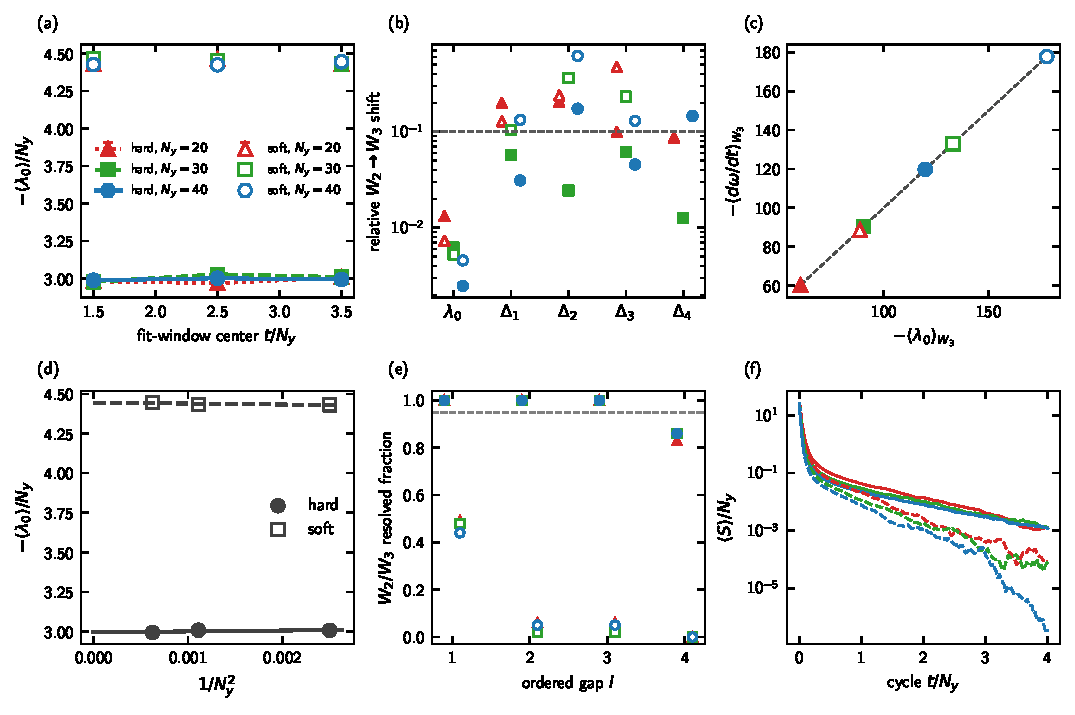
\includegraphics[width=\textwidth]{figure_assets/purification_lyapunov_main.pdf}
 \caption{Many-body Lyapunov and purification analysis.  Each point uses
 $S=100$ independent maximally mixed Born trajectories at fixed $N_y$; lines
 and filled symbols denote hard walls and open symbols or dashed lines denote
 soft walls.  Error bars in (a) and (c) are trajectory standard errors.
 (a) Window-resolved leading free-energy density.  (b) Magnitude of the paired
 $W_2\to W_3$ shift; the dashed line is the 10\% magnitude condition, while
 acceptance additionally requires a paired 95\% bootstrap interval containing
 zero and 95\% numerical resolution.  (c) Same-$W_3$ record-weight and leading
 spectral slopes; the dashed line is equality.  (d) Three-size $1/N_y^2$ fits.
 (e) Fraction of trajectories numerically resolving each ordered gap through
 both $W_2$ and $W_3$; the dashed line is the 95\% requirement.  (f) Total
 entropy per circumference through $T=4N_y$.  Fits are trajectory-first and
 bootstrap intervals use 2000 whole-trajectory replicates.}
 \label{fig:main}
\end{figure*}

\subsection{Censored excited spectrum}

The longer evolution creates a precision boundary for the excited spectrum.
In the hard arm the first three gaps remain resolved for all trajectories in
$W_2$ and $W_3$, whereas the fourth is resolved for only 83--86\%.  In the
soft arm the first gap is resolved for 44--49\%, the second and third for only
2--6\%, and the fourth for none.  This is consistent with the much more
complete soft-wall purification, but it prevents an unbiased late-window soft
gap fit in complex128.  Fitting only the surviving less-purified records would
condition on the outcome and bias the ensemble, so the missing values are
reported as censored.

For the hard arm, $\Delta_3$ is the only ordered gap passing the complete
temporal, resolution, positive-coefficient, and 20\% finite-size sensitivity
gates.  Its descriptive coefficient is
\begin{equation}
 A_3=4.827\ [4.453,5.194],\qquad
 \alpha x_3=0.768\ [0.709,0.827].
\end{equation}
This is a provisional ordered-gap coefficient, not an identified operator
dimension.  The files contain occupation eigenvalues but not their natural
eigenvectors, momentum, charge-sector, or two-wall symmetry labels.  The
index ``3'' therefore denotes sorted order only.

\subsection{Finite-size coefficient}

Following Eqs.~(3) and (4) of Zabalo \emph{et al.}, we fit
\begin{align}
 -\frac{\lambda_0}{N_y}
 &=f_\infty+\frac{A_0}{N_y^2},\\
 \frac{\lambda_0-\lambda_i}{N_y}
 &=\frac{A_i}{N_y^2}.
\end{align}
The leading hard-wall result is
\begin{equation}
 A_0=+5.59\ [-15.19,26.98],
\end{equation}
and the soft-wall result is
\begin{equation}
 A_0=-6.13\ [-29.21,17.20].
\end{equation}
Both intervals contain zero.  Adding the exactly determined $1/N_y^4$ term
changes $A_0$ to $59.7$ and $-51.7$, while omitting $N_y=20$ changes it to
$30.7$ and $-27.2$.  These are sensitivity factors of 9.70 and 7.45 relative
to the primary coefficients, far above 20\%.  The formal diagnostics
$\alpha c_{\rm eff}=-10.7$ and $+11.7$ are consequently rejected rather than
reported as physical estimates.  Three circumferences cannot separate a
universal $1/N_y^2$ term from subleading structure at the observed noise level.

Random without-replacement $S=25,50,75$ subsets retain broad, sign-changing
$A_0$ distributions.  Increasing samples alone is therefore not the obvious
next repair; additional circumferences or an independently constrained
finite-size form are needed.

\subsection{Purification and spatial residuals}

At $4N_y$, the mean hard-wall entropy is $0.0249$, $0.0393$, and $0.0474$ at
$N_y=20,30,40$; the corresponding charge variances are $0.00706$, $0.0113$,
and $0.0134$.  Approximately 96.2--96.5\% of both residuals lies in the fixed
three-column windows around $x=5$ and $x=15$.  The soft-wall endpoint entropy
is $1.67\times10^{-3}$, $2.46\times10^{-3}$, and $1.47\times10^{-5}$; its
charge variance is $3.77\times10^{-4}$, $5.87\times10^{-4}$, and
$1.25\times10^{-6}$.  About 94.8--95.6\% of the soft charge variance remains
in the wall windows.  The soft entropy fraction is less stable because its
denominator is already nearly zero.  These contours localize residual
mixedness; they do not localize individual singular modes.

\begin{figure*}[t]
 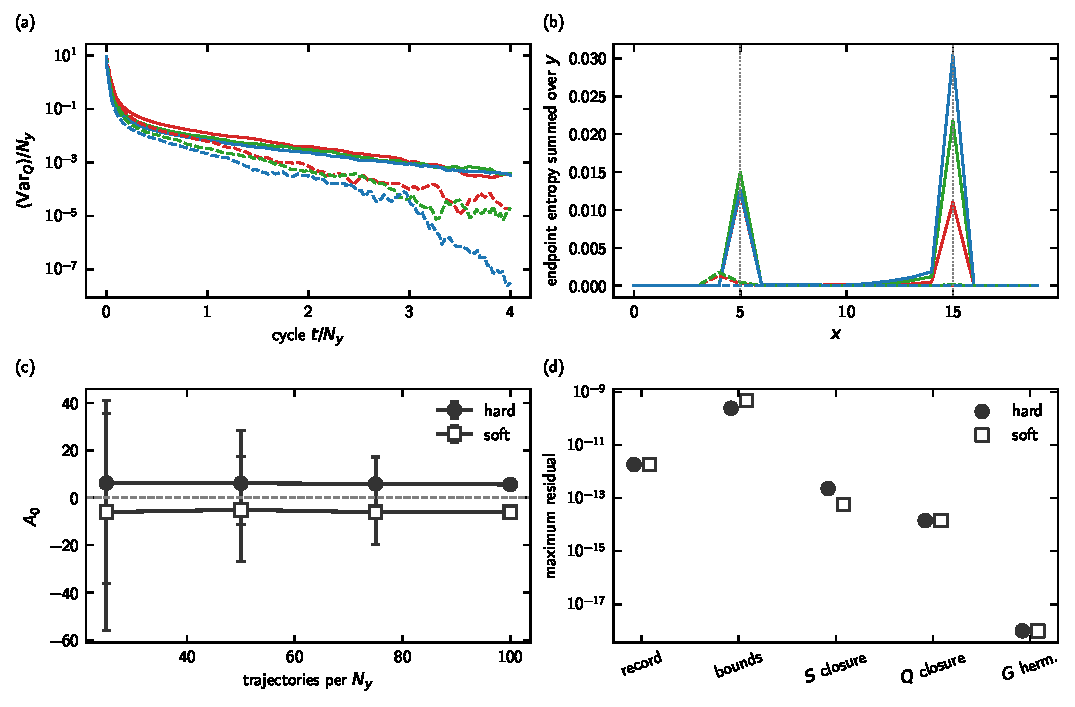
\includegraphics[width=\textwidth]{figure_assets/purification_lyapunov_diagnostics.pdf}
 \caption{Numerical and purification diagnostics for the same $S=100$,
 $T=4N_y$ independent-trajectory ensembles.  (a) Total intrinsic charge
 variance per circumference.  (b) Endpoint entropy profiles summed along the
 periodic direction; dotted vertical lines mark the domain walls at $x=5,15$.
 (c) Random without-replacement sample convergence of $A_0$; error bars for
 $S<100$ are central 95\% intervals across 200 subsets, while $S=100$ is the
 unique full ensemble.  (d) Maximum record, occupation-bound, entropy-closure,
 charge-closure, and final-covariance Hermiticity residuals.  Colors encode
 $N_y=20,30,40$ as red triangles, green squares, and blue circles.}
 \label{fig:diagnostics}
\end{figure*}

\section{Claim ledger and interpretation}

The completed analysis supports four statements.  First, the Gaussian
occupation spectrum and record weight reconstruct an absolute many-body
singular spectrum with controlled normalization.  Second, $\lambda_0$ reaches
a stable late-time window by $4N_y$.  Third, residual entropy and charge
variance are concentrated near the two interfaces.  Fourth, one hard-wall
ordered-gap coefficient survives the preregistered numerical gates as a
descriptive quantity.

It does not support a precision $c_{\rm eff}$, absolute $x_i$, or a conformal
tower assignment.  The anisotropy $\alpha$ is not independently calibrated,
the circumference grid has only three points, and the soft excited spectrum is
precision-censored.  The already established spatial evidence for boundary
criticality is useful context, but it cannot rescue an unstable independent
Lyapunov finite-size coefficient.  The discrepancy is a finite-size and
numerical-resolution limitation, not a failure of the boundary-critical state.

\section{Reproducibility}

The machine-readable directory accompanying this note contains trajectory
window slopes, temporal and record-closure ledgers, finite-size and sample-size
fits, cycle summaries, endpoint profiles, shardwise numerical diagnostics, and
\texttt{analysis\_summary.json}.  The analysis command is
\begin{verbatim}
python analyze_completed_campaign.py
\end{verbatim}
from bundle 07.  Production acceptance requires the default checksum pass;
the development-only \texttt{--skip-file-hashes} option is not used for the
final report.  The bootstrap seed is 2026090907.

\section{Conclusion}

The $4N_y$ data answer the primary depth question.  The leading many-body
Lyapunov rate and absolute record normalization have converged at all three
circumferences for both hard and soft walls.  The remaining obstruction is not
trajectory count or leading-time convergence: it is the narrow three-size grid
for $A_0$ and, for soft-wall excitations, double-precision censoring after near
complete purification.  The defensible paper result is therefore a validated
absolute Gaussian spectrum and stable leading rate, accompanied by a clear
negative result for precision CFT coefficient extraction.

\end{document}
